\section{Video Compression}
\label{sec:introduction/section_b}

The early form of video compression was described by Ray Davis Kell in 1929, as the difficulty of transmitting successive images of video can be avoided by only sending the difference between the successive images, though it was not actually used; however, it became the foundation for the video compression standards today \cite{jacobs_brief_2009}. Early video compression was analog, but digital video processing has been developed and is widely used today. \citeauthor{zhang_overview_2019} \cite{zhang_overview_2019} explained the concept of typical video compression nowadays as following. The video compression consists of the encoder compressing the images into the compressed form, which can be stored or transmitted to another location, and the decoder to decompress the images. This process of coding and decoding is also called a codec. Typical video compression standards nowadays comprise predictive coding, transform coding, and entropy coding, as shown in Figure \ref{fig:comp_architecture}. Predictive coding is the component that reduces the inter-frame temporal redundancy and intra-frame spatial redundancy in a video by motion estimation (ME), motion compensation (MC), and spatial prediction techniques. Transform coding is the component where the quantized transform coefficients are generated through discrete cosine transform (DCT) to help reduce the spatial redundancy. Entropy coding is the component where compressed bitstreams are generated.

\begin{figure}[!tb]
  \centering
  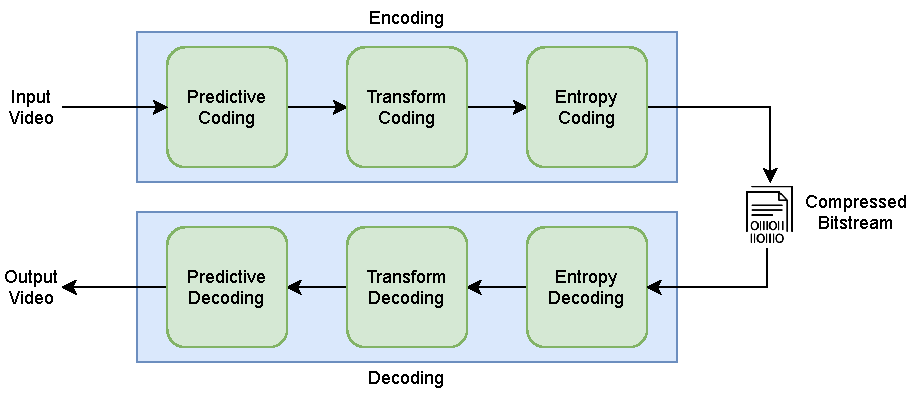
\includegraphics[width=0.8\linewidth]{img/comp_architecture.pdf}
  \caption[The typical video compression architecture]
  {
  The typical video compression architecture adapted from \cite{zhang_overview_2019}.
%   The encoder consists of predictive coding, transform coding, and entropy coding compresses the input video and generates the compressed bitstream. The decoder decompresses the bitstream in reverse order to the encoder and outputs the reconstructed video.
  }
  \label{fig:comp_architecture}
\end{figure}

There are two types of video coding: lossless coding and lossy coding. Lossless coding compresses the images and obtains the reconstructed images after decompression without any loss of information. Lossy coding, however, compresses the images by removing the less important information, which will sacrifice the image quality to the level the human visual system can tolerate. Lossy compression is more widely used today since it allows a much smaller compressed size and is more efficient than the lossless compression.

Since the first video compression standard H.120 developed in 1984, various video compression standards have been developed, such as MPEG and H.26X series \cite{zhang_overview_2019}. They all followed the architecture shown in Figure \ref{fig:comp_architecture}. The organization of Moving Picture Experts Group (MPEG) in the International Standards Organization (ISO) and the International Electrotechnical Commission (IEC) are developing the MPEG series such as MPEG-1, MPEG-2, and MPEG-4.

The Video Coding Expert Group (VCEG) of the International Telecommunication Union (ITU-T) is developing H.26X series starting from the first standard H.120. They subsequently developed H.261, H.262, H.263, H.264 (AVC), and H.265 (HEVC). H.264, so-called Advanced Video Coding (AVC), was released in 2003. H.264/AVC is the most widely used standard nowadays and supports up to 4k resolution of video. H.265, so-called High Efficiency Video Coding (HEVC), was developed based on H.264/AVC structure and is a more recent standard that has been released in 2013. H.265/HEVC supports up to 8k resolution of the video but is not yet widely supported. There has been more recent development of standards such as, for example, Versatile Video Coding (VVC) and AOMedia Video 1 (AV1). These newly developed standards, after the predecessor of H.265/HEVC, achieve better coding performance and will allow high quality and efficiency, virtual reality (VR) system, and 360-degree video applications. However, these standards and H.265/HEVC are still yet to be supported due to the current hardware's lack of computational power. As a possible future generation of video compression standards after VVC and AV1, there has been research in compression technologies utilizing machine learning for video coding, hardware acceleration, and parallel computing. Out of these video compression standards, we have adopted H.265/HEVC for the experiments in this thesis.